\documentclass[]{article}
\usepackage{lmodern}
\usepackage{amssymb,amsmath}
\usepackage{ifxetex,ifluatex}
\usepackage{fixltx2e} % provides \textsubscript
\ifnum 0\ifxetex 1\fi\ifluatex 1\fi=0 % if pdftex
  \usepackage[T1]{fontenc}
  \usepackage[utf8]{inputenc}
\else % if luatex or xelatex
  \ifxetex
    \usepackage{mathspec}
  \else
    \usepackage{fontspec}
  \fi
  \defaultfontfeatures{Ligatures=TeX,Scale=MatchLowercase}
\fi
% use upquote if available, for straight quotes in verbatim environments
\IfFileExists{upquote.sty}{\usepackage{upquote}}{}
% use microtype if available
\IfFileExists{microtype.sty}{%
\usepackage{microtype}
\UseMicrotypeSet[protrusion]{basicmath} % disable protrusion for tt fonts
}{}
\usepackage[margin=1in]{geometry}
\usepackage{hyperref}
\hypersetup{unicode=true,
            pdfborder={0 0 0},
            breaklinks=true}
\urlstyle{same}  % don't use monospace font for urls
\usepackage{color}
\usepackage{fancyvrb}
\newcommand{\VerbBar}{|}
\newcommand{\VERB}{\Verb[commandchars=\\\{\}]}
\DefineVerbatimEnvironment{Highlighting}{Verbatim}{commandchars=\\\{\}}
% Add ',fontsize=\small' for more characters per line
\usepackage{framed}
\definecolor{shadecolor}{RGB}{248,248,248}
\newenvironment{Shaded}{\begin{snugshade}}{\end{snugshade}}
\newcommand{\KeywordTok}[1]{\textcolor[rgb]{0.13,0.29,0.53}{\textbf{#1}}}
\newcommand{\DataTypeTok}[1]{\textcolor[rgb]{0.13,0.29,0.53}{#1}}
\newcommand{\DecValTok}[1]{\textcolor[rgb]{0.00,0.00,0.81}{#1}}
\newcommand{\BaseNTok}[1]{\textcolor[rgb]{0.00,0.00,0.81}{#1}}
\newcommand{\FloatTok}[1]{\textcolor[rgb]{0.00,0.00,0.81}{#1}}
\newcommand{\ConstantTok}[1]{\textcolor[rgb]{0.00,0.00,0.00}{#1}}
\newcommand{\CharTok}[1]{\textcolor[rgb]{0.31,0.60,0.02}{#1}}
\newcommand{\SpecialCharTok}[1]{\textcolor[rgb]{0.00,0.00,0.00}{#1}}
\newcommand{\StringTok}[1]{\textcolor[rgb]{0.31,0.60,0.02}{#1}}
\newcommand{\VerbatimStringTok}[1]{\textcolor[rgb]{0.31,0.60,0.02}{#1}}
\newcommand{\SpecialStringTok}[1]{\textcolor[rgb]{0.31,0.60,0.02}{#1}}
\newcommand{\ImportTok}[1]{#1}
\newcommand{\CommentTok}[1]{\textcolor[rgb]{0.56,0.35,0.01}{\textit{#1}}}
\newcommand{\DocumentationTok}[1]{\textcolor[rgb]{0.56,0.35,0.01}{\textbf{\textit{#1}}}}
\newcommand{\AnnotationTok}[1]{\textcolor[rgb]{0.56,0.35,0.01}{\textbf{\textit{#1}}}}
\newcommand{\CommentVarTok}[1]{\textcolor[rgb]{0.56,0.35,0.01}{\textbf{\textit{#1}}}}
\newcommand{\OtherTok}[1]{\textcolor[rgb]{0.56,0.35,0.01}{#1}}
\newcommand{\FunctionTok}[1]{\textcolor[rgb]{0.00,0.00,0.00}{#1}}
\newcommand{\VariableTok}[1]{\textcolor[rgb]{0.00,0.00,0.00}{#1}}
\newcommand{\ControlFlowTok}[1]{\textcolor[rgb]{0.13,0.29,0.53}{\textbf{#1}}}
\newcommand{\OperatorTok}[1]{\textcolor[rgb]{0.81,0.36,0.00}{\textbf{#1}}}
\newcommand{\BuiltInTok}[1]{#1}
\newcommand{\ExtensionTok}[1]{#1}
\newcommand{\PreprocessorTok}[1]{\textcolor[rgb]{0.56,0.35,0.01}{\textit{#1}}}
\newcommand{\AttributeTok}[1]{\textcolor[rgb]{0.77,0.63,0.00}{#1}}
\newcommand{\RegionMarkerTok}[1]{#1}
\newcommand{\InformationTok}[1]{\textcolor[rgb]{0.56,0.35,0.01}{\textbf{\textit{#1}}}}
\newcommand{\WarningTok}[1]{\textcolor[rgb]{0.56,0.35,0.01}{\textbf{\textit{#1}}}}
\newcommand{\AlertTok}[1]{\textcolor[rgb]{0.94,0.16,0.16}{#1}}
\newcommand{\ErrorTok}[1]{\textcolor[rgb]{0.64,0.00,0.00}{\textbf{#1}}}
\newcommand{\NormalTok}[1]{#1}
\usepackage{longtable,booktabs}
\usepackage{graphicx,grffile}
\makeatletter
\def\maxwidth{\ifdim\Gin@nat@width>\linewidth\linewidth\else\Gin@nat@width\fi}
\def\maxheight{\ifdim\Gin@nat@height>\textheight\textheight\else\Gin@nat@height\fi}
\makeatother
% Scale images if necessary, so that they will not overflow the page
% margins by default, and it is still possible to overwrite the defaults
% using explicit options in \includegraphics[width, height, ...]{}
\setkeys{Gin}{width=\maxwidth,height=\maxheight,keepaspectratio}
\IfFileExists{parskip.sty}{%
\usepackage{parskip}
}{% else
\setlength{\parindent}{0pt}
\setlength{\parskip}{6pt plus 2pt minus 1pt}
}
\setlength{\emergencystretch}{3em}  % prevent overfull lines
\providecommand{\tightlist}{%
  \setlength{\itemsep}{0pt}\setlength{\parskip}{0pt}}
\setcounter{secnumdepth}{0}
% Redefines (sub)paragraphs to behave more like sections
\ifx\paragraph\undefined\else
\let\oldparagraph\paragraph
\renewcommand{\paragraph}[1]{\oldparagraph{#1}\mbox{}}
\fi
\ifx\subparagraph\undefined\else
\let\oldsubparagraph\subparagraph
\renewcommand{\subparagraph}[1]{\oldsubparagraph{#1}\mbox{}}
\fi

%%% Use protect on footnotes to avoid problems with footnotes in titles
\let\rmarkdownfootnote\footnote%
\def\footnote{\protect\rmarkdownfootnote}

%%% Change title format to be more compact
\usepackage{titling}

% Create subtitle command for use in maketitle
\providecommand{\subtitle}[1]{
  \posttitle{
    \begin{center}\large#1\end{center}
    }
}

\setlength{\droptitle}{-2em}

  \title{}
    \pretitle{\vspace{\droptitle}}
  \posttitle{}
    \author{}
    \preauthor{}\postauthor{}
    \date{}
    \predate{}\postdate{}
  

\begin{document}

{
\setcounter{tocdepth}{1}
\tableofcontents
}
\begin{center}
\includegraphics[width=0.6\linewidth]{aalto} \end{center}

\begin{verbatim}
FALSE Loading required package: StanHeaders
\end{verbatim}

\begin{verbatim}
FALSE Loading required package: ggplot2
\end{verbatim}

\begin{verbatim}
FALSE rstan (Version 2.19.2, GitRev: 2e1f913d3ca3)
\end{verbatim}

\begin{verbatim}
FALSE For execution on a local, multicore CPU with excess RAM we recommend calling
FALSE options(mc.cores = parallel::detectCores()).
FALSE To avoid recompilation of unchanged Stan programs, we recommend calling
FALSE rstan_options(auto_write = TRUE)
\end{verbatim}

\begin{verbatim}
FALSE For improved execution time, we recommend calling
FALSE Sys.setenv(LOCAL_CPPFLAGS = '-march=native')
FALSE although this causes Stan to throw an error on a few processors.
\end{verbatim}

\begin{verbatim}
FALSE This is loo version 2.1.0.
FALSE **NOTE: As of version 2.0.0 loo defaults to 1 core but we recommend using as many as possible. Use the 'cores' argument or set options(mc.cores = NUM_CORES) for an entire session. Visit mc-stan.org/loo/news for details on other changes.
\end{verbatim}

\begin{verbatim}
FALSE **NOTE for Windows 10 users: loo may be very slow if 'mc.cores' is set in your .Rprofile file (see https://github.com/stan-dev/loo/issues/94).
\end{verbatim}

\begin{verbatim}
FALSE 
FALSE Attaching package: 'loo'
\end{verbatim}

\begin{verbatim}
FALSE The following object is masked from 'package:rstan':
FALSE 
FALSE     loo
\end{verbatim}

\begin{verbatim}
FALSE Loading required package: Rcpp
\end{verbatim}

\begin{verbatim}
FALSE rstanarm (Version 2.19.2, packaged: 2019-10-01 20:20:33 UTC)
\end{verbatim}

\begin{verbatim}
FALSE - Do not expect the default priors to remain the same in future rstanarm versions.
\end{verbatim}

\begin{verbatim}
FALSE Thus, R scripts should specify priors explicitly, even if they are just the defaults.
\end{verbatim}

\begin{verbatim}
FALSE - For execution on a local, multicore CPU with excess RAM we recommend calling
\end{verbatim}

\begin{verbatim}
FALSE options(mc.cores = parallel::detectCores())
\end{verbatim}

\begin{verbatim}
FALSE - bayesplot theme set to bayesplot::theme_default()
\end{verbatim}

\begin{verbatim}
FALSE    * Does _not_ affect other ggplot2 plots
\end{verbatim}

\begin{verbatim}
FALSE    * See ?bayesplot_theme_set for details on theme setting
\end{verbatim}

\begin{verbatim}
FALSE 
FALSE Attaching package: 'rstanarm'
\end{verbatim}

\begin{verbatim}
FALSE The following object is masked from 'package:rstan':
FALSE 
FALSE     loo
\end{verbatim}

\begin{verbatim}
FALSE This is bayesplot version 1.7.0
\end{verbatim}

\begin{verbatim}
FALSE - Online documentation and vignettes at mc-stan.org/bayesplot
\end{verbatim}

\begin{verbatim}
FALSE - bayesplot theme set to bayesplot::theme_default()
\end{verbatim}

\begin{verbatim}
FALSE    * Does _not_ affect other ggplot2 plots
\end{verbatim}

\begin{verbatim}
FALSE    * See ?bayesplot_theme_set for details on theme setting
\end{verbatim}

\begin{verbatim}
FALSE Parsed with column specification:
FALSE cols(
FALSE   year = col_double(),
FALSE   state = col_character(),
FALSE   month = col_character(),
FALSE   number = col_double(),
FALSE   date = col_date(format = "")
FALSE )
\end{verbatim}

\section{1 Abstract}\label{abstract}

The aim of this project is to analyze the number of fires in the states
of Brazil and build a Bayesian model in order to make predictions about
the frequency of forest fires in a time series can help to take action
to prevent them.

\section{2 Introduction}\label{introduction}

The dataset on which the analysis are made is taken from ``Kaggle'', an
online community of data scientists and machine learners where many data
sets are available for the users. The ``amazon'' dataset reports the
number of forest fires in Brazil divided by states. The series comprises
the period of approximately 10 years (1998 to 2017). The data were
obtained from the official website of the Brazilian government. Brazil
has the largest rainforest on the planet that is the Amazon rainforest.
Forest fires are a serious problem for the preservation of the Tropical
Forests. Understanding the frequency of forest fires in a time series
can help to take action to prevent them.

\section{3 Explorative Analysis}\label{explorative-analysis}

In the original dataset ``Amazon'', the following features are present:

\begin{itemize}
\tightlist
\item
  year (1998 - 2017);
\item
  state (23);
\item
  month;
\item
  number;
\item
  date;
\end{itemize}

All the following analysis are made on a subset of the initial dataset.
For each state and for each year, the sum of the total fires per month
is calculated. Say also x and y in order to apply the models.

The dataset can be visualized in the below map. The intensity of the
colour is proportional to the mean number of fires among the years 1998
- 2017, as displayed in the legend on the right.

\begin{figure}
\centering
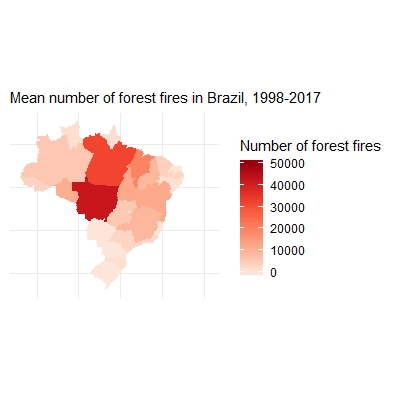
\includegraphics{brazilmap_1.jpeg}
\caption{Number of fires - Brazil}
\end{figure}

In this dataset there is a big eterogeneity between the states. In the
following boxplots, the mean and the variability between the number of
fires in each state are displayed.

\begin{center}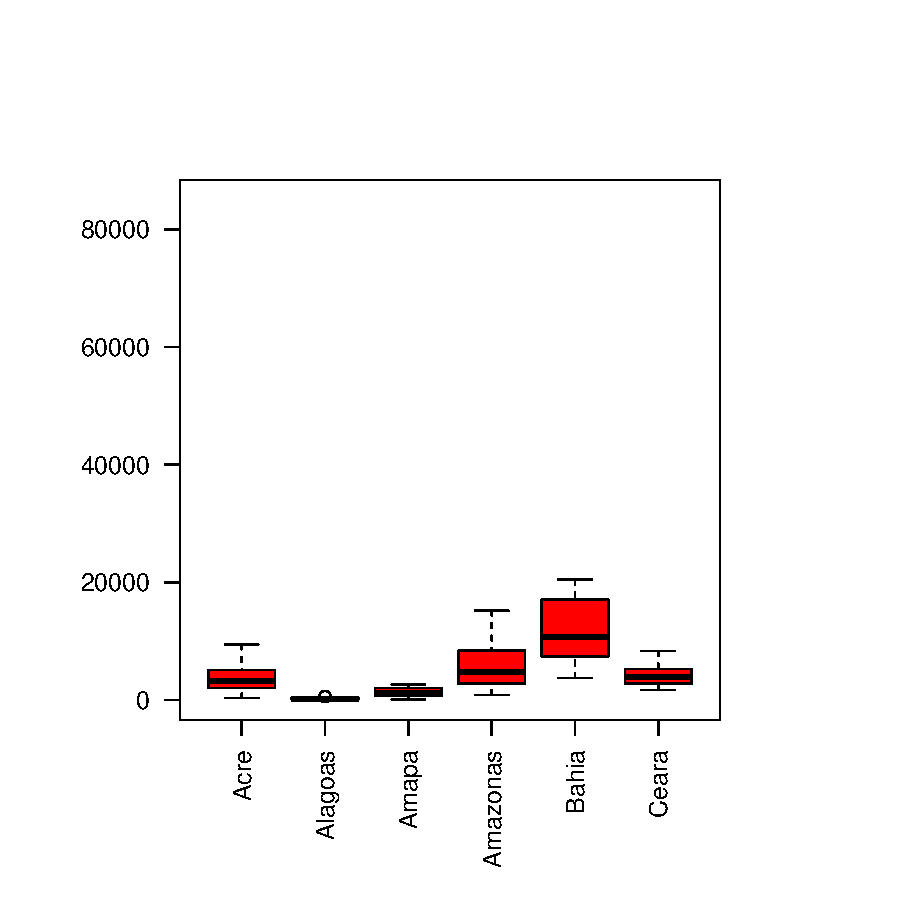
\includegraphics[width=.49\linewidth]{Data_science_project_files/figure-latex/unnamed-chunk-5-1} 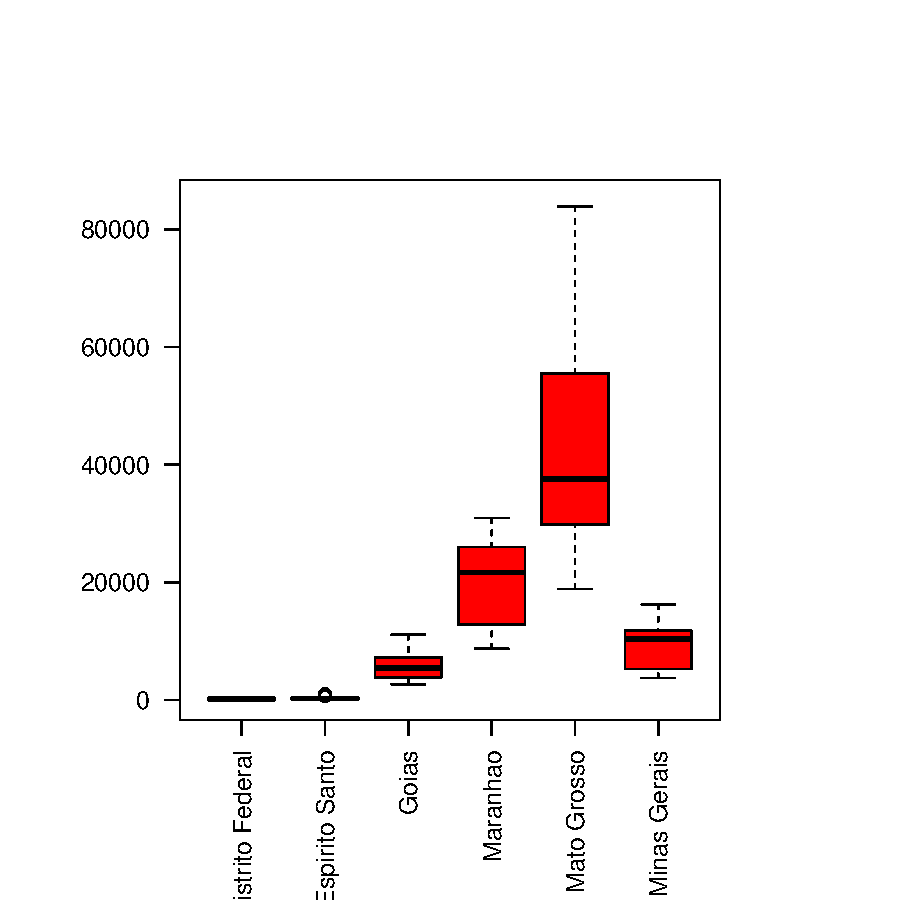
\includegraphics[width=.49\linewidth]{Data_science_project_files/figure-latex/unnamed-chunk-5-2} \end{center}

\begin{center}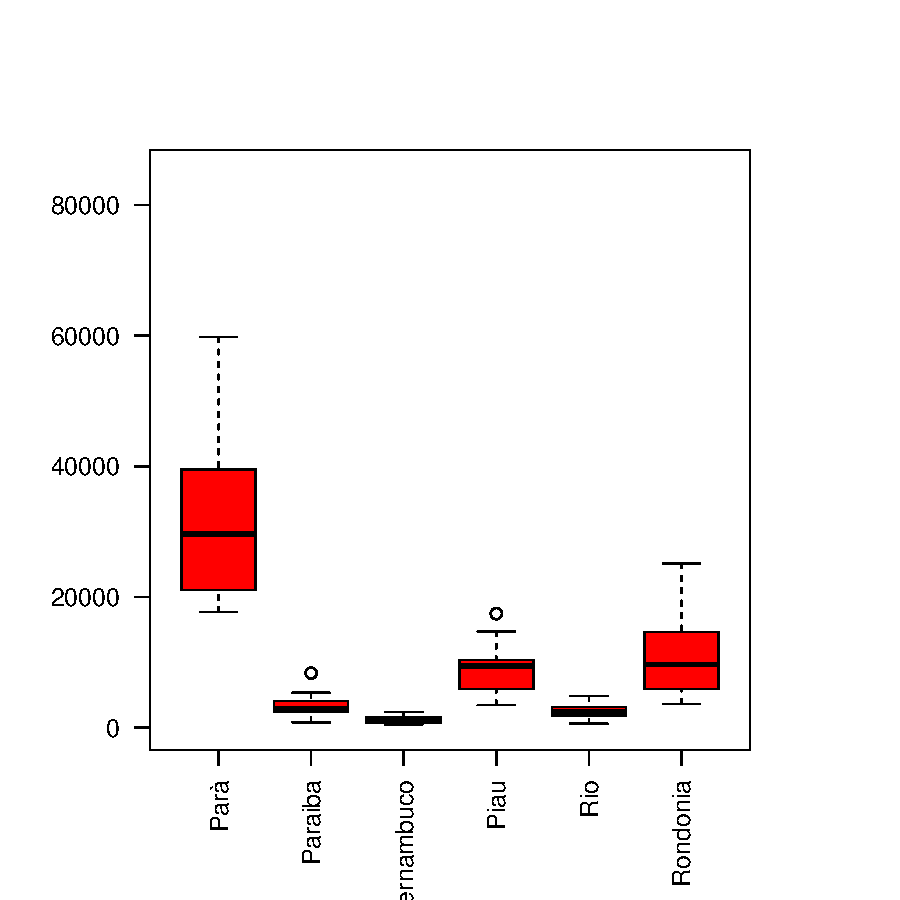
\includegraphics[width=.49\linewidth]{Data_science_project_files/figure-latex/unnamed-chunk-6-1} 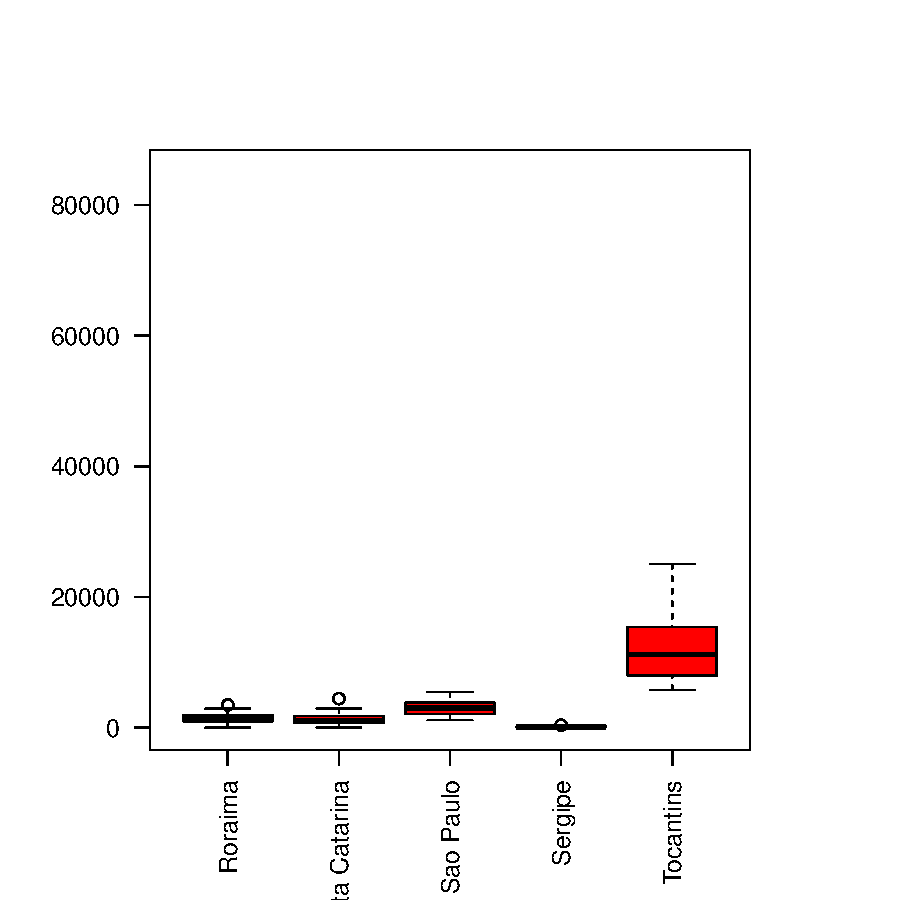
\includegraphics[width=.49\linewidth]{Data_science_project_files/figure-latex/unnamed-chunk-6-2} \end{center}

Moreover, in the following matplot every line corresponds to a different
state. The y-axes represents the number of fires for that state while
the x-axes represent the years (from 1998 to 2017). It can be seen that
there is not a linear increasing of the number of fires among the years.

\begin{center}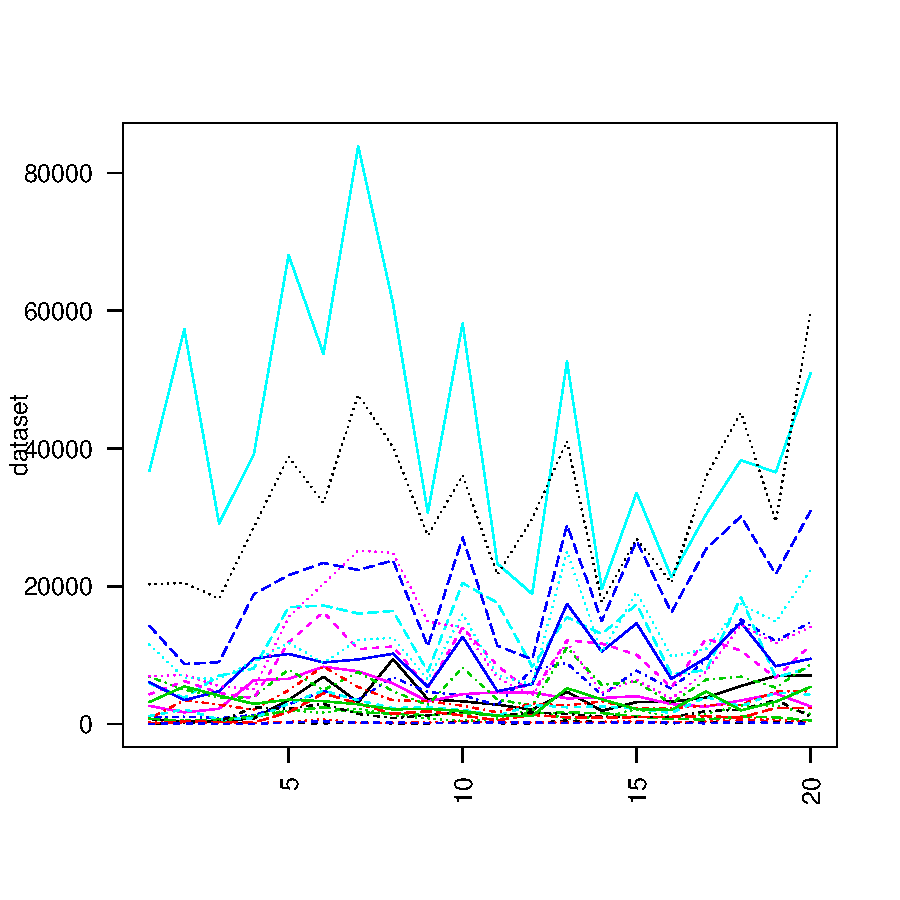
\includegraphics[width=.49\linewidth]{Data_science_project_files/figure-latex/unnamed-chunk-7-1} \end{center}

\section{4 Methods}\label{methods}

\subsection{4.1 Choice of models}\label{choice-of-models}

Because of the hierarchical structure of the data, building a
hierarchical model was a natural choice. Since there are massive
differences in variance and mean between the states, a pooled model can
not perform very well in analyzing a single state. Because of this, we
have focused on comparing separate and hierarchical models.

First, a normal model is introduced, as it is a good basis to build
further models on and it provides a good baseline for further results.
Because of the aforementioned qualities of the dataset (mean and
variance) the next model we built was a negative binomial model, which
should fit the dataset better. A separate and hierarchical versions of
this model proved to model our data better than their normal
counterparts. The last model we included was a regression model that
utilizes the negative binomial distribution and predicts the amount of
fires for the year 2018 in each of the states.

We also experimented with additional models that we decided to leave out
because of their poor performance or the lack of sensible results. These
models include a poisson model, pooled versions of the used models, and
regression models that use a different distribution or alternative
parametrizations that stan provides.

\subsection{4.2 Choice of priors}\label{choice-of-priors}

We wanted to capture the large variance in the dataset with our choice
of priors. For the normal models we used a prior distribution
\(\mu_0 ~ N(\mu, \sigma)\), where \(\mu\) is the mean of the dataset and
\(\sigma\) is the variance of the dataset.

For the negative binomial model, as well as the regression model, we
used the priors \(\alpha u\) and \(\beta = 1.2\)

\subsection{4.3 Methods for comparing the
models}\label{methods-for-comparing-the-models}

\section{5 Experiments and Results}\label{experiments-and-results}

\subsection{5.1 Normal Model}\label{normal-model}

\subsection{5.1.1 Separate Normal Model}\label{separate-normal-model}

\[ y_{ji} \sim N(\mu_j,\sigma_j)\]

\begin{Shaded}
\begin{Highlighting}[]
\CommentTok{# DEFINITION OF THE SEPARATE MODEL IN STAN}

\NormalTok{separate_code =}\StringTok{ "}

\StringTok{data \{}
\StringTok{  int<lower=0> N;             // number of data points}
\StringTok{  int<lower=0> K;             // number of groups}
\StringTok{  int<lower=1,upper=K> x[N];  // group indicator}
\StringTok{  vector[N] y;}
\StringTok{\}}

\StringTok{parameters \{}
\StringTok{  vector[K] mu;               // group means}
\StringTok{  vector<lower=0>[K] sigma;   // group stds}
\StringTok{\}}

\StringTok{model \{}
\StringTok{  y ~ normal(mu[x], sigma[x]);}
\StringTok{\}}

\StringTok{generated quantities \{}
\StringTok{  vector[K] y_state;}
\StringTok{  vector[N] log_lik;                                }

\StringTok{  for (i in 1:N)                                           }
\StringTok{    log_lik[i] = normal_lpdf(y[i] | mu[x[i]], sigma[x[i]]);     }
\StringTok{  }
\StringTok{  for (i in 1:K)}
\StringTok{    y_state[i]=normal_rng(mu[i], sigma[i]);}
\StringTok{\}}

\StringTok{"}
\end{Highlighting}
\end{Shaded}

\subsection{5.1.2 Pooled Normal Model}\label{pooled-normal-model}

\[ y_i \sim N(\mu,\sigma)\]

\begin{Shaded}
\begin{Highlighting}[]
\CommentTok{# DEFINITION OF THE POOLED MODEL IN STAN}

\NormalTok{pooled_code =}\StringTok{ "}

\StringTok{data \{}
\StringTok{  int<lower=0> N;      // number of data points}
\StringTok{  vector[N] y;         //}
\StringTok{\}}

\StringTok{parameters \{}
\StringTok{  real mu;             // common mean}
\StringTok{  real<lower=0> sigma; // common std}
\StringTok{\}}

\StringTok{model \{}
\StringTok{  y ~ normal(mu, sigma);}
\StringTok{\}}


\StringTok{generated quantities \{ }
\StringTok{  real ypred;}
\StringTok{  vector[N] log_lik;}
\StringTok{  ypred = normal_rng(mu,sigma);}
\StringTok{  for (i in 1:N)}
\StringTok{    log_lik[i] = normal_lpdf(y[i] | mu, sigma);   }
\StringTok{\}}
\StringTok{"}
\end{Highlighting}
\end{Shaded}

\subsection{5.1.3 Hierarchical Normal
Model}\label{hierarchical-normal-model}

\[ y_{ji} \sim N(\overline{\mu}+\mu_j,\sigma)\]

\begin{Shaded}
\begin{Highlighting}[]
\CommentTok{# DEFINITION OF HIERARCHICAL MODEL IN STAN }

\NormalTok{hierarchical_code =}\StringTok{ "}

\StringTok{data \{}
\StringTok{  int<lower=0> N;           // number of data points}
\StringTok{  int<lower=0> K;           // number of groups}
\StringTok{  int<lower=1,upper=K> x[N]; // group indicator}
\StringTok{  vector[N] y;              }
\StringTok{\}}

\StringTok{parameters \{}
\StringTok{  real mu0;                 // prior mean}
\StringTok{  real<lower=0> sigma0;     // prior std}
\StringTok{  vector[K] mu;             // group means}
\StringTok{  real<lower=0> sigma;      // common std}
\StringTok{\}}

\StringTok{model \{}

\StringTok{  mu0 ~ normal(7933,25325);  // weakly informative prior}
\StringTok{  sigma0 ~ cauchy(0,4);      // weakly informative prior}
\StringTok{  mu ~ normal(mu0, sigma0);  // population prior with unknown parameters}
\StringTok{  sigma ~ cauchy(0,4);       // weakly informative prior}
\StringTok{  y ~ normal(mu[x], sigma);}
\StringTok{\}}

\StringTok{generated quantities \{}
\StringTok{  real ypred;}
\StringTok{  real mupred;}
\StringTok{  vector[K] y_state;}
\StringTok{  vector[N] log_lik; }

\StringTok{  mupred = normal_rng(mu0,sigma0);}
\StringTok{  ypred = normal_rng(mupred, sigma);}
\StringTok{  }
\StringTok{  for (i in 1:N) }
\StringTok{    log_lik[i] = normal_lpdf(y[i] | mu[x[i]], sigma); }

\StringTok{  for (i in 1:K)}
\StringTok{    y_state[i]=normal_rng(mu[i], sigma);}

\StringTok{\}}
\StringTok{"}
\end{Highlighting}
\end{Shaded}

\begin{verbatim}
## Warning: There were 34 divergent transitions after warmup. Increasing adapt_delta above 0.8 may help. See
## http://mc-stan.org/misc/warnings.html#divergent-transitions-after-warmup
\end{verbatim}

\begin{verbatim}
## Warning: There were 263 transitions after warmup that exceeded the maximum treedepth. Increase max_treedepth above 10. See
## http://mc-stan.org/misc/warnings.html#maximum-treedepth-exceeded
\end{verbatim}

\begin{verbatim}
## Warning: Examine the pairs() plot to diagnose sampling problems
\end{verbatim}

\begin{verbatim}
## Warning: The largest R-hat is 1.58, indicating chains have not mixed.
## Running the chains for more iterations may help. See
## http://mc-stan.org/misc/warnings.html#r-hat
\end{verbatim}

\begin{verbatim}
## Warning: Bulk Effective Samples Size (ESS) is too low, indicating posterior means and medians may be unreliable.
## Running the chains for more iterations may help. See
## http://mc-stan.org/misc/warnings.html#bulk-ess
\end{verbatim}

\begin{verbatim}
## Warning: Tail Effective Samples Size (ESS) is too low, indicating posterior variances and tail quantiles may be unreliable.
## Running the chains for more iterations may help. See
## http://mc-stan.org/misc/warnings.html#tail-ess
\end{verbatim}

\subsection{5.1.4 Results of the Normal
Models}\label{results-of-the-normal-models}

Here we have computed the PSIS-LOO elpd values and the k-values for each
of the three normal models introduced in the last section as well as the
effective number of parameters Peff for each of the three models.

\begin{Shaded}
\begin{Highlighting}[]
\CommentTok{# SEPARATE MODEL}
\NormalTok{loo_separate=}\KeywordTok{loo}\NormalTok{(fit_separate)}
\end{Highlighting}
\end{Shaded}

\begin{verbatim}
## Warning: Some Pareto k diagnostic values are too high. See help('pareto-k-diagnostic') for details.
\end{verbatim}

\begin{Shaded}
\begin{Highlighting}[]
\KeywordTok{plot}\NormalTok{(loo_separate)}
\end{Highlighting}
\end{Shaded}

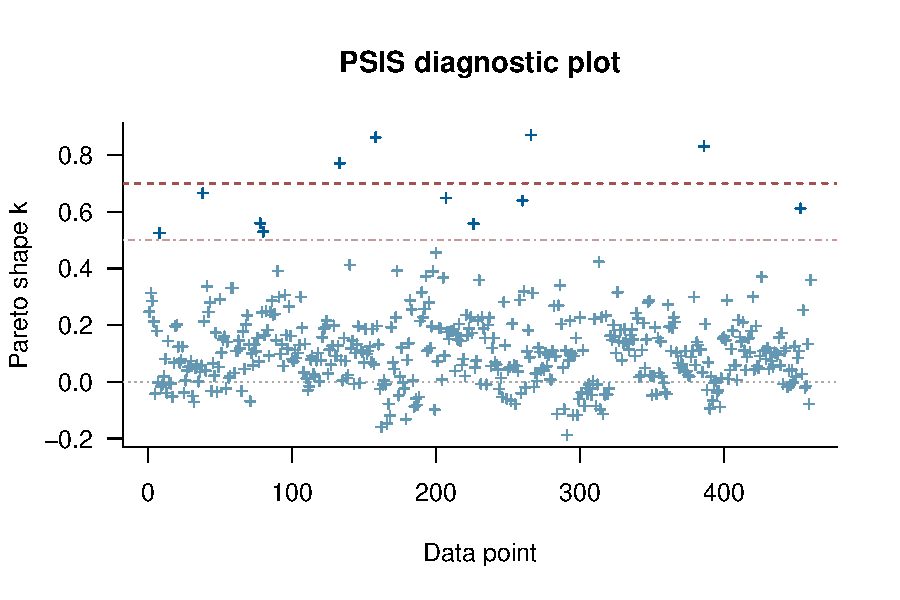
\includegraphics{Data_science_project_files/figure-latex/unnamed-chunk-14-1.pdf}

\begin{Shaded}
\begin{Highlighting}[]
\NormalTok{log_lik_s <-}\StringTok{ }\KeywordTok{extract_log_lik}\NormalTok{(fit_separate, }\DataTypeTok{merge_chains =} \OtherTok{FALSE}\NormalTok{)}
\NormalTok{r_eff_s <-}\StringTok{ }\KeywordTok{relative_eff}\NormalTok{(}\KeywordTok{exp}\NormalTok{(log_lik_s))}
\NormalTok{loo_s <-}\StringTok{ }\KeywordTok{loo}\NormalTok{(log_lik_s, }\DataTypeTok{r_eff =}\NormalTok{ r_eff_s, }\DataTypeTok{save_psis=}\OtherTok{TRUE}\NormalTok{, }\DataTypeTok{cores=}\DecValTok{2}\NormalTok{ )}
\end{Highlighting}
\end{Shaded}

\begin{verbatim}
## Warning: Some Pareto k diagnostic values are too high. See help('pareto-k-diagnostic') for details.
\end{verbatim}

\begin{Shaded}
\begin{Highlighting}[]
\KeywordTok{print}\NormalTok{(loo_s)}
\end{Highlighting}
\end{Shaded}

\begin{verbatim}
## 
## Computed from 4000 by 460 log-likelihood matrix
## 
##          Estimate   SE
## elpd_loo  -4088.3 34.9
## p_loo        44.9  5.3
## looic      8176.5 69.8
## ------
## Monte Carlo SE of elpd_loo is NA.
## 
## Pareto k diagnostic values:
##                          Count Pct.    Min. n_eff
## (-Inf, 0.5]   (good)     448   97.4%   545       
##  (0.5, 0.7]   (ok)         8    1.7%   75        
##    (0.7, 1]   (bad)        4    0.9%   30        
##    (1, Inf)   (very bad)   0    0.0%   <NA>      
## See help('pareto-k-diagnostic') for details.
\end{verbatim}

\begin{Shaded}
\begin{Highlighting}[]
\CommentTok{# POOLED MODEL}
\NormalTok{loo_pooled=}\KeywordTok{loo}\NormalTok{(fit_pooled) }
\KeywordTok{plot}\NormalTok{(loo_pooled)}
\end{Highlighting}
\end{Shaded}

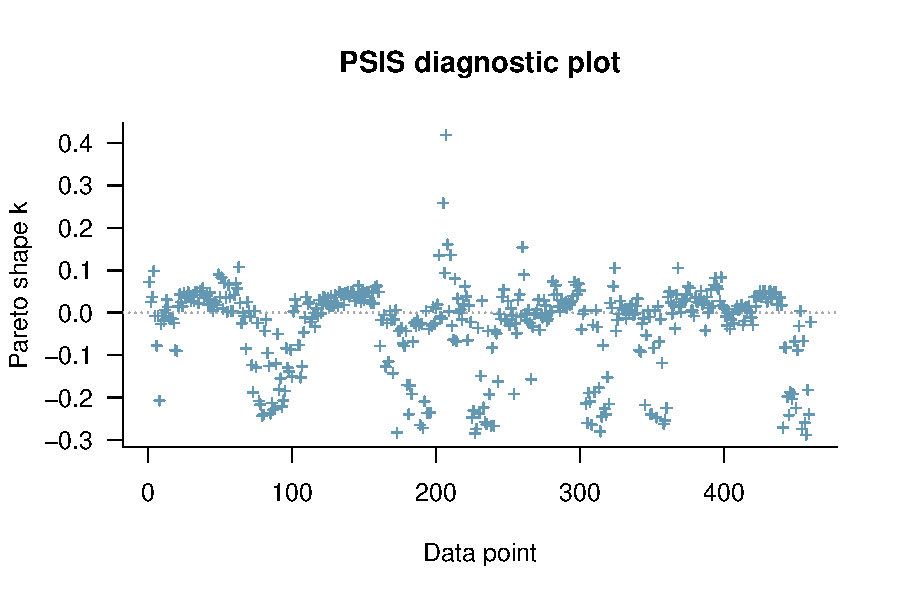
\includegraphics{Data_science_project_files/figure-latex/unnamed-chunk-14-2.pdf}

\begin{Shaded}
\begin{Highlighting}[]
\NormalTok{log_lik_p <-}\StringTok{ }\KeywordTok{extract_log_lik}\NormalTok{(fit_pooled, }\DataTypeTok{merge_chains =} \OtherTok{FALSE}\NormalTok{)}
\NormalTok{r_eff_p <-}\StringTok{ }\KeywordTok{relative_eff}\NormalTok{(}\KeywordTok{exp}\NormalTok{(log_lik_p))}
\NormalTok{loo_p <-}\StringTok{ }\KeywordTok{loo}\NormalTok{(log_lik_p, }\DataTypeTok{r_eff =}\NormalTok{ r_eff_p, }\DataTypeTok{save_psis=}\OtherTok{TRUE}\NormalTok{, }\DataTypeTok{cores=}\DecValTok{2}\NormalTok{ )}
\KeywordTok{print}\NormalTok{(loo_p)}
\end{Highlighting}
\end{Shaded}

\begin{verbatim}
## 
## Computed from 4000 by 460 log-likelihood matrix
## 
##          Estimate   SE
## elpd_loo  -4962.2 37.0
## p_loo         6.4  2.2
## looic      9924.4 74.0
## ------
## Monte Carlo SE of elpd_loo is 0.1.
## 
## All Pareto k estimates are good (k < 0.5).
## See help('pareto-k-diagnostic') for details.
\end{verbatim}

\begin{Shaded}
\begin{Highlighting}[]
\CommentTok{# HIERARCHICAL MODEL - normal}
\NormalTok{loo_hierarchical=}\KeywordTok{loo}\NormalTok{(fit_hierarchical)}
\end{Highlighting}
\end{Shaded}

\begin{verbatim}
## Warning: Some Pareto k diagnostic values are too high. See help('pareto-k-diagnostic') for details.
\end{verbatim}

\begin{Shaded}
\begin{Highlighting}[]
\KeywordTok{plot}\NormalTok{(loo_hierarchical)}

\NormalTok{log_lik_h <-}\StringTok{ }\KeywordTok{extract_log_lik}\NormalTok{(fit_hierarchical, }\DataTypeTok{merge_chains =} \OtherTok{FALSE}\NormalTok{)}
\NormalTok{r_eff_h <-}\StringTok{ }\KeywordTok{relative_eff}\NormalTok{(}\KeywordTok{exp}\NormalTok{(log_lik_h))}
\NormalTok{loo_h <-}\StringTok{ }\KeywordTok{loo}\NormalTok{(log_lik_h, }\DataTypeTok{r_eff =}\NormalTok{ r_eff_h, }\DataTypeTok{save_psis=}\OtherTok{TRUE}\NormalTok{, }\DataTypeTok{cores=}\DecValTok{2}\NormalTok{ )}
\end{Highlighting}
\end{Shaded}

\begin{verbatim}
## Warning: Some Pareto k diagnostic values are too high. See help('pareto-k-diagnostic') for details.
\end{verbatim}

\begin{Shaded}
\begin{Highlighting}[]
\KeywordTok{print}\NormalTok{(loo_h)}
\end{Highlighting}
\end{Shaded}

\begin{verbatim}
## 
## Computed from 4000 by 460 log-likelihood matrix
## 
##          Estimate   SE
## elpd_loo  -4781.8 47.6
## p_loo       152.4 19.3
## looic      9563.7 95.3
## ------
## Monte Carlo SE of elpd_loo is NA.
## 
## Pareto k diagnostic values:
##                          Count Pct.    Min. n_eff
## (-Inf, 0.5]   (good)     441   95.9%   0         
##  (0.5, 0.7]   (ok)        10    2.2%   0         
##    (0.7, 1]   (bad)        8    1.7%   5         
##    (1, Inf)   (very bad)   1    0.2%   0         
## See help('pareto-k-diagnostic') for details.
\end{verbatim}

\begin{Shaded}
\begin{Highlighting}[]
\KeywordTok{plot}\NormalTok{(loo_h)}
\end{Highlighting}
\end{Shaded}

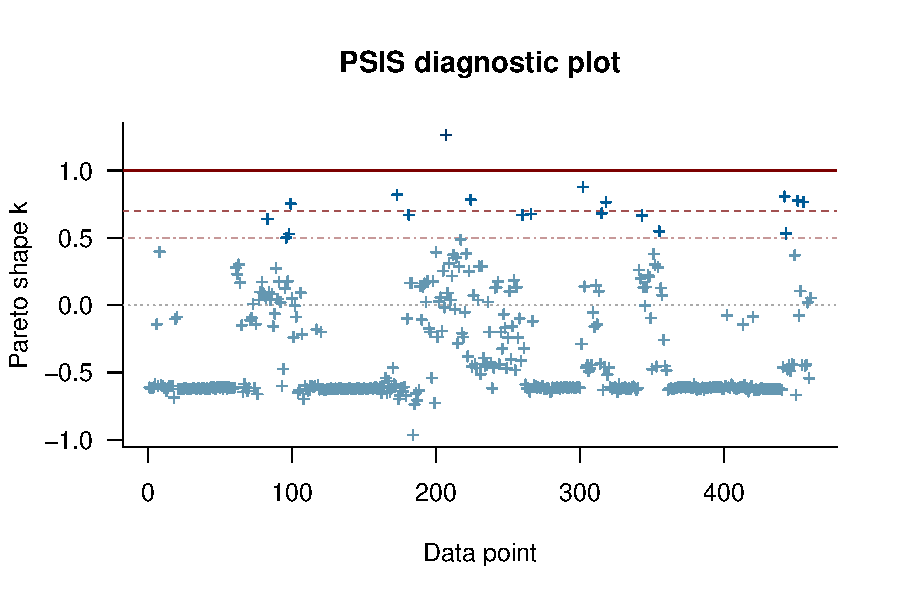
\includegraphics{Data_science_project_files/figure-latex/unnamed-chunk-14-3.pdf}

\begin{Shaded}
\begin{Highlighting}[]
\CommentTok{# ESTIMATION OF PSIS-LOO values }

\NormalTok{loo_s}\OperatorTok{$}\NormalTok{estimates[}\DecValTok{1}\NormalTok{] }\CommentTok{#separate}
\end{Highlighting}
\end{Shaded}

\begin{verbatim}
## [1] -4088.252
\end{verbatim}

\begin{Shaded}
\begin{Highlighting}[]
\NormalTok{loo_p}\OperatorTok{$}\NormalTok{estimates[}\DecValTok{1}\NormalTok{] }\CommentTok{#pooled}
\end{Highlighting}
\end{Shaded}

\begin{verbatim}
## [1] -4962.186
\end{verbatim}

\begin{Shaded}
\begin{Highlighting}[]
\NormalTok{loo_h}\OperatorTok{$}\NormalTok{estimates[}\DecValTok{1}\NormalTok{] }\CommentTok{#hierarchical - normal}
\end{Highlighting}
\end{Shaded}

\begin{verbatim}
## [1] -4781.836
\end{verbatim}

Next, we have computed the effective number of parameters Peff for each
of the three models.

Answer: Equation (7.15) in the book:
\[ p_{loo-cv} = lppd - lppd_{loo-cv} \] where

\[ lppd_{loo-cv} \] is the PSIS-LOO value (sum of the LOO log densities)
(calculated above in point 2)

and
\[ lppd = \sum_{i=1}^n \log( \frac{1}{S} \sum_{s=1}^S p(y_i|\theta^s))\]
The lppd of the observed data y is an overestimate of the elppd for
future data.

\begin{Shaded}
\begin{Highlighting}[]
\NormalTok{S=}\DecValTok{4000}
\NormalTok{n=}\DecValTok{20}\OperatorTok{*}\DecValTok{23}

\CommentTok{# ESTIMATION OF lppd}

\CommentTok{# SEPARATE}
\NormalTok{vector_s=}\KeywordTok{rep}\NormalTok{(}\DecValTok{0}\NormalTok{,n)}
\ControlFlowTok{for}\NormalTok{(i }\ControlFlowTok{in} \DecValTok{1}\OperatorTok{:}\NormalTok{n)}
\NormalTok{ vector_s[i]=}\KeywordTok{log}\NormalTok{(}\DecValTok{1}\OperatorTok{/}\NormalTok{S}\OperatorTok{*}\NormalTok{(}\KeywordTok{sum}\NormalTok{(}\KeywordTok{exp}\NormalTok{(samples_s}\OperatorTok{$}\NormalTok{log_lik[,i]))))}

\CommentTok{# POOLED}
\NormalTok{vector_p=}\KeywordTok{rep}\NormalTok{(}\DecValTok{0}\NormalTok{,n)}
\ControlFlowTok{for}\NormalTok{(i }\ControlFlowTok{in} \DecValTok{1}\OperatorTok{:}\NormalTok{n)}
\NormalTok{ vector_p[i]=}\KeywordTok{log}\NormalTok{(}\DecValTok{1}\OperatorTok{/}\NormalTok{S}\OperatorTok{*}\NormalTok{(}\KeywordTok{sum}\NormalTok{(}\KeywordTok{exp}\NormalTok{(samples_p}\OperatorTok{$}\NormalTok{log_lik[,i]))))}


\CommentTok{# HIERARCHICAL - normal}
\NormalTok{vector_h=}\KeywordTok{rep}\NormalTok{(}\DecValTok{0}\NormalTok{,n)}
\ControlFlowTok{for}\NormalTok{(i }\ControlFlowTok{in} \DecValTok{1}\OperatorTok{:}\NormalTok{n)}
\NormalTok{ vector_h[i]=}\KeywordTok{log}\NormalTok{(}\DecValTok{1}\OperatorTok{/}\NormalTok{S}\OperatorTok{*}\NormalTok{(}\KeywordTok{sum}\NormalTok{(}\KeywordTok{exp}\NormalTok{(samples_h}\OperatorTok{$}\NormalTok{log_lik[,i]))))}
\end{Highlighting}
\end{Shaded}

\begin{Shaded}
\begin{Highlighting}[]
\CommentTok{#RESULTING VALUES FOR peff}

\NormalTok{peff_s =}\StringTok{ }\KeywordTok{sum}\NormalTok{(vector_s) }\OperatorTok{-}\StringTok{ }\NormalTok{loo_s}\OperatorTok{$}\NormalTok{estimates[}\DecValTok{1}\NormalTok{]}
\NormalTok{peff_p =}\StringTok{ }\KeywordTok{sum}\NormalTok{(vector_p) }\OperatorTok{-}\NormalTok{loo_p}\OperatorTok{$}\NormalTok{estimates[}\DecValTok{1}\NormalTok{]}
\NormalTok{peff_h =}\StringTok{ }\KeywordTok{sum}\NormalTok{(vector_h) }\OperatorTok{-}\StringTok{ }\NormalTok{loo_h}\OperatorTok{$}\NormalTok{estimates[}\DecValTok{1}\NormalTok{]}

\NormalTok{peff_s }\CommentTok{#separate}
\end{Highlighting}
\end{Shaded}

\begin{verbatim}
## [1] 44.91247
\end{verbatim}

\begin{Shaded}
\begin{Highlighting}[]
\NormalTok{peff_p }\CommentTok{#pooled}
\end{Highlighting}
\end{Shaded}

\begin{verbatim}
## [1] 6.430996
\end{verbatim}

\begin{Shaded}
\begin{Highlighting}[]
\NormalTok{peff_h }\CommentTok{#hierarchical normal}
\end{Highlighting}
\end{Shaded}

\begin{verbatim}
## [1] 152.356
\end{verbatim}

\subsection{5.2.1 Separate Negative Binomial
Model}\label{separate-negative-binomial-model}

As discussed in the methods section of this document, the data has a
higher variance than mean. Because of this we applied a negative
binomial model to the data.

\begin{Shaded}
\begin{Highlighting}[]
\NormalTok{separate_negative_bin =}\StringTok{ "}

\StringTok{data \{}
\StringTok{  int<lower=0> N;           // number of data points}
\StringTok{  int<lower=0> K;           // number of groups}
\StringTok{  int<lower=1,upper=K> x[N]; // group indicator}
\StringTok{  int<lower=0> y[N];              }
\StringTok{\}}

\StringTok{parameters \{}
\StringTok{  real<lower=0> alpha[K]; }
\StringTok{  real<lower=0> beta[K];}
\StringTok{\}}

\StringTok{model \{}
\StringTok{  alpha ~ exponential(0.0006303); //change this}
\StringTok{  beta ~ exponential(1.2); }
\StringTok{  y ~ neg_binomial(alpha[x], beta[x]);}
\StringTok{\}}

\StringTok{generated quantities \{}
\StringTok{  int<lower=0> y_rep[K]; }
\StringTok{  vector[N] log_lik; }
\StringTok{  }
\StringTok{  for (i in 1:N) }
\StringTok{    log_lik[i] = neg_binomial_lpmf(y[i] | alpha[x[i]], beta[x[i]]);}

\StringTok{  for (i in 1:K) }
\StringTok{    y_rep[i] = neg_binomial_rng(alpha[i], beta[i]); }
\StringTok{\}}
\StringTok{"}
\end{Highlighting}
\end{Shaded}

\subsection{5.2.2 Hierarchical Negative Binomial
Model}\label{hierarchical-negative-binomial-model}

\begin{Shaded}
\begin{Highlighting}[]
 \CommentTok{# DEFINITION OF THE HIERARCHICAL MODEL IN STAN}

\NormalTok{hierarchical_negative_bin =}\StringTok{ "}

\StringTok{data \{}
\StringTok{  int<lower=0> N;           // number of data points}
\StringTok{  int<lower=0> K;           // number of groups}
\StringTok{  int<lower=1,upper=K> x[N]; // group indicator}
\StringTok{  int<lower=0> y[N];              }
\StringTok{\}}

\StringTok{parameters \{}
\StringTok{  real alpha;}
\StringTok{  real<lower=0> beta[K]; }
\StringTok{\}}

\StringTok{model \{}
\StringTok{  alpha ~ exponential(0.0006303);}
\StringTok{  beta ~ exponential(1.2); }
\StringTok{  y ~ neg_binomial(alpha, beta[x]);}
\StringTok{\}}

\StringTok{generated quantities \{}
\StringTok{  int<lower=0> y_rep[K]; }
\StringTok{  vector[N] log_lik; }
\StringTok{  }
\StringTok{  for (i in 1:N) }
\StringTok{    log_lik[i] = neg_binomial_lpmf(y[i] | alpha, beta[x[i]]);}

\StringTok{  for (i in 1:K) }
\StringTok{    y_rep[i] = neg_binomial_rng(alpha, beta[i]); }
\StringTok{\}}
\StringTok{"}
\end{Highlighting}
\end{Shaded}

\subsection{5.2.3 Results of the Negative Binomial
Models}\label{results-of-the-negative-binomial-models}

\begin{Shaded}
\begin{Highlighting}[]
\CommentTok{# Separate Model}
\NormalTok{samples_s =}\StringTok{ }\KeywordTok{extract}\NormalTok{(}\DataTypeTok{object=}\NormalTok{separate_neg_binomial_fit, }\DataTypeTok{permuted =} \OtherTok{TRUE}\NormalTok{, }\DataTypeTok{inc_warmup =} \OtherTok{FALSE}\NormalTok{, }\DataTypeTok{include =} \OtherTok{TRUE}\NormalTok{)}

\NormalTok{log_lik_s <-}\StringTok{ }\KeywordTok{extract_log_lik}\NormalTok{(separate_neg_binomial_fit, }\DataTypeTok{merge_chains =} \OtherTok{FALSE}\NormalTok{)}
\NormalTok{r_eff_s <-}\StringTok{ }\KeywordTok{relative_eff}\NormalTok{(}\KeywordTok{exp}\NormalTok{(log_lik_s))}
\NormalTok{loo_model_s <-}\StringTok{ }\KeywordTok{loo}\NormalTok{(log_lik_s, }\DataTypeTok{r_eff =}\NormalTok{ r_eff_s, }\DataTypeTok{save_psis=}\OtherTok{TRUE}\NormalTok{, }\DataTypeTok{cores=}\DecValTok{2}\NormalTok{ )}
\end{Highlighting}
\end{Shaded}

\begin{verbatim}
## Warning: Some Pareto k diagnostic values are slightly high. See help('pareto-k-diagnostic') for details.
\end{verbatim}

\begin{Shaded}
\begin{Highlighting}[]
\KeywordTok{print}\NormalTok{(loo_model_s)}
\end{Highlighting}
\end{Shaded}

\begin{verbatim}
## 
## Computed from 4000 by 80 log-likelihood matrix
## 
##          Estimate   SE
## elpd_loo   -665.8 14.4
## p_loo         8.7  1.7
## looic      1331.7 28.8
## ------
## Monte Carlo SE of elpd_loo is 0.1.
## 
## Pareto k diagnostic values:
##                          Count Pct.    Min. n_eff
## (-Inf, 0.5]   (good)     79    98.8%   441       
##  (0.5, 0.7]   (ok)        1     1.2%   278       
##    (0.7, 1]   (bad)       0     0.0%   <NA>      
##    (1, Inf)   (very bad)  0     0.0%   <NA>      
## 
## All Pareto k estimates are ok (k < 0.7).
## See help('pareto-k-diagnostic') for details.
\end{verbatim}

\begin{Shaded}
\begin{Highlighting}[]
\KeywordTok{plot}\NormalTok{(loo_model_s)}
\end{Highlighting}
\end{Shaded}

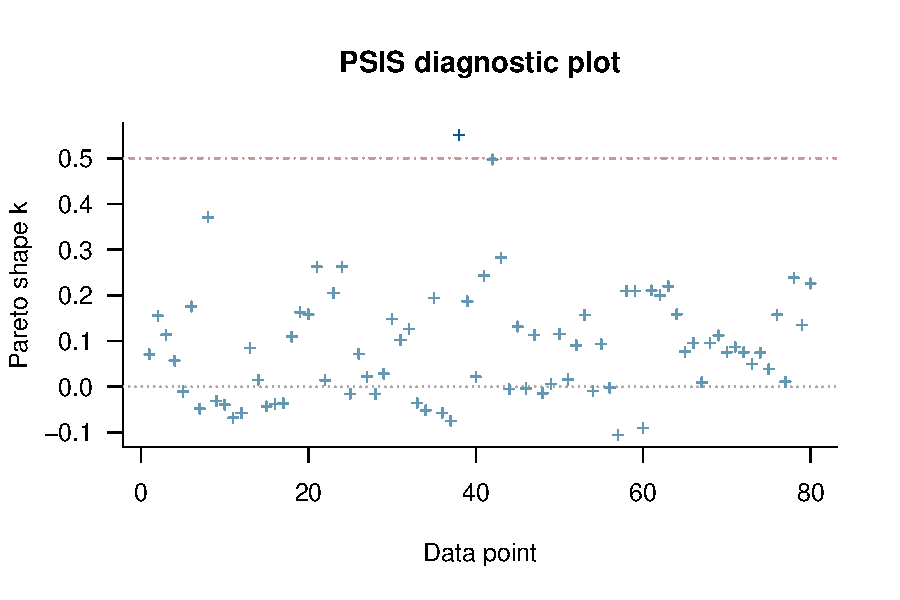
\includegraphics{Data_science_project_files/figure-latex/unnamed-chunk-22-1.pdf}

\begin{Shaded}
\begin{Highlighting}[]
\CommentTok{# PSIS-LOO values}
\NormalTok{loo_model_s}\OperatorTok{$}\NormalTok{estimates[}\DecValTok{1}\NormalTok{] }
\end{Highlighting}
\end{Shaded}

\begin{verbatim}
## [1] -665.832
\end{verbatim}

\begin{Shaded}
\begin{Highlighting}[]
\CommentTok{# Hierarchical Model}
\NormalTok{samples_h =}\StringTok{ }\KeywordTok{extract}\NormalTok{(}\DataTypeTok{object=}\NormalTok{hierarchical_neg_binomial_fit, }\DataTypeTok{permuted =} \OtherTok{TRUE}\NormalTok{, }\DataTypeTok{inc_warmup =} \OtherTok{FALSE}\NormalTok{, }\DataTypeTok{include =} \OtherTok{TRUE}\NormalTok{)}

\NormalTok{log_lik_h <-}\StringTok{ }\KeywordTok{extract_log_lik}\NormalTok{(hierarchical_neg_binomial_fit, }\DataTypeTok{merge_chains =} \OtherTok{FALSE}\NormalTok{)}
\NormalTok{r_eff_h <-}\StringTok{ }\KeywordTok{relative_eff}\NormalTok{(}\KeywordTok{exp}\NormalTok{(log_lik_h))}
\NormalTok{loo_model_h <-}\StringTok{ }\KeywordTok{loo}\NormalTok{(log_lik_h, }\DataTypeTok{r_eff =}\NormalTok{ r_eff_h, }\DataTypeTok{save_psis=}\OtherTok{TRUE}\NormalTok{, }\DataTypeTok{cores=}\DecValTok{2}\NormalTok{ )}
\KeywordTok{print}\NormalTok{(loo_model_h)}
\end{Highlighting}
\end{Shaded}

\begin{verbatim}
## 
## Computed from 4000 by 460 log-likelihood matrix
## 
##          Estimate   SE
## elpd_loo  -4062.9 36.3
## p_loo        24.3  2.1
## looic      8125.8 72.7
## ------
## Monte Carlo SE of elpd_loo is 0.1.
## 
## All Pareto k estimates are good (k < 0.5).
## See help('pareto-k-diagnostic') for details.
\end{verbatim}

\begin{Shaded}
\begin{Highlighting}[]
\KeywordTok{plot}\NormalTok{(loo_model_h)}
\end{Highlighting}
\end{Shaded}

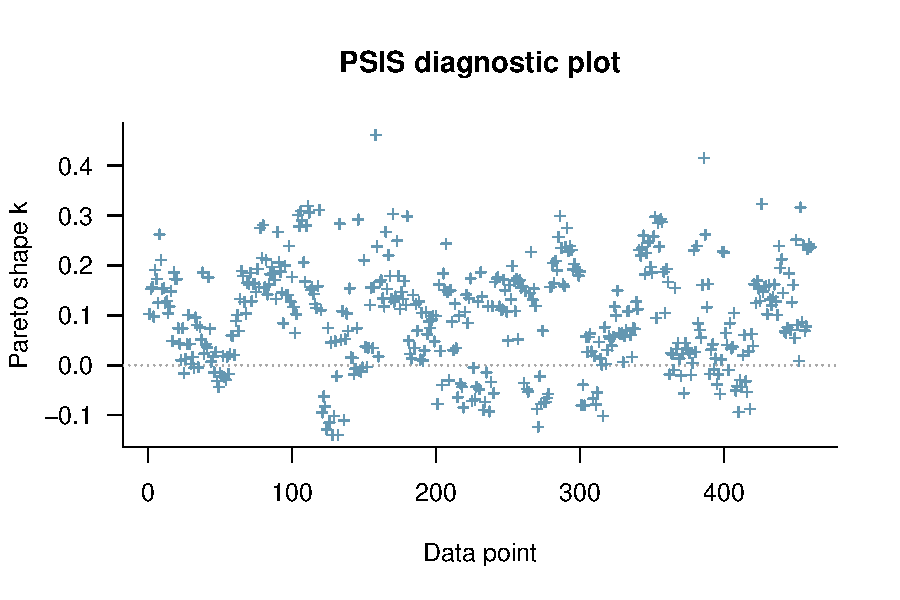
\includegraphics{Data_science_project_files/figure-latex/unnamed-chunk-22-2.pdf}

\begin{Shaded}
\begin{Highlighting}[]
\CommentTok{# PSIS-LOO values}
\NormalTok{loo_model_h}\OperatorTok{$}\NormalTok{estimates[}\DecValTok{1}\NormalTok{]}
\end{Highlighting}
\end{Shaded}

\begin{verbatim}
## [1] -4062.895
\end{verbatim}

\subsection{5.3.1 Hierarchical Regression
Model}\label{hierarchical-regression-model}

\begin{Shaded}
\begin{Highlighting}[]
\CommentTok{# DEFINITION OF THE MODEL IN STAN}

\NormalTok{hierarchical_regression =}\StringTok{ "}

\StringTok{data \{}
\StringTok{  int<lower=0> N;     //number of datapoints}
\StringTok{  int<lower=0> K;     //number of groups}
\StringTok{  vector[N] x;        //predictor (year)}
\StringTok{  int<lower=0> y[N];  //response (n of fires)}
\StringTok{  real xpred;         //regression predictor}
\StringTok{\}}
\StringTok{parameters \{}
\StringTok{  real<lower=0> alpha;}
\StringTok{  real<lower=0> beta;}
\StringTok{  real<lower=0> phi;}
\StringTok{\}}
\StringTok{model \{}
\StringTok{  phi ~ exponential(1.2);}
\StringTok{  alpha ~ exponential(0.0006303);}
\StringTok{  beta ~ exponential(0.0006303);}
\StringTok{  y ~ neg_binomial(alpha + beta * x, phi);}
\StringTok{\}}

\StringTok{generated quantities \{}
\StringTok{  int<lower=0> ypred[K];}
\StringTok{  vector[N] log_lik;}
\StringTok{  }
\StringTok{  for (i in 1:K) }
\StringTok{    ypred[i] = neg_binomial_rng(alpha + beta * xpred, phi);}
\StringTok{  }
\StringTok{  for (i in 1:N) }
\StringTok{    log_lik[i] = neg_binomial_lpmf(y[i] | alpha, beta);}
\StringTok{\}}
\StringTok{"}
\end{Highlighting}
\end{Shaded}

\begin{longtable}[]{@{}lrrr@{}}
\caption{Comparison between the two best fitted models}\tabularnewline
\toprule
& ME & ME\_ratio & MSE\tabularnewline
\midrule
\endfirsthead
\toprule
& ME & ME\_ratio & MSE\tabularnewline
\midrule
\endhead
LINEAR - reduced & 72.036 & 24.36812 & 501.0531\tabularnewline
MIXED - reduced & 68.743 & 23.25400 & 535.1980\tabularnewline
\bottomrule
\end{longtable}

\section{Reference}\label{reference}

\begin{itemize}
\item
  \url{https://www.kaggle.com/gustavomodelli/forest-fires-in-brazil}
\item
  \url{https://datascienceplus.com/bayesian-regression-with-stan-beyond-normality/}
\item
  \url{https://mc-stan.org/docs/2_20/functions-reference/nbalt.html}
\item
  \url{https://mc-stan.org/loo/reference/loo-glossary.html}
\item ~
  \section{\texorpdfstring{\url{https://github.com/avehtari/BDA_R_demos/blob/master/demos_rstan/ppc/poisson-simple.stan}}{https://github.com/avehtari/BDA\_R\_demos/blob/master/demos\_rstan/ppc/poisson-simple.stan}}\label{httpsgithub.comavehtaribda_r_demosblobmasterdemos_rstanppcpoisson-simple.stan}
\end{itemize}


\end{document}
